\subsection{In-Situ High-Speed Computer Vision}
{{\footnotesize
\noindent Applies low-latency CNN models for image classification of plasma diagnostics streams; supports deployment on embedded platforms.


\begin{description}[labelwidth=4cm, labelsep=1em, leftmargin=4cm, itemsep=0.1em, parsep=0em]
  \item[date:] 2023-12-05
  \item[version:] v1.0
  \item[last\_updated:] 2023-12
  \item[expired:] unknown
  \item[valid:] yes
  \item[valid\_date:] 2023-12-05
  \item[url:] \href{https://arxiv.org/abs/2312.00128}{https://arxiv.org/abs/2312.00128}
  \item[doi:] 10.48550/arXiv.2312.00128
  \item[domain:]
    - High Energy Physics
  \item[focus:] Real-time image classification for in-situ plasma diagnostics
  \item[keywords:]
    - plasma
    - in-situ vision
    - real-time ML
  \item[licensing:] Via Fermilab
  \item[task\_types:]
    - Image Classification
  \item[ai\_capability\_measured:]
    - Real-time diagnostic inference
  \item[metrics:]
    - Accuracy
    - FPS
  \item[models:]
    - CNN
  \item[ml\_motif:]
    - Classification
  \item[type:] Model
  \item[ml\_task:]
    - Image Classification
  \item[solutions:] Solution details are described in the referenced paper or repository.
  \item[notes:] Embedded/deployment details in progress.

  \item[contact.name:] unknown
  \item[contact.email:] unknown
  \item[results.links.name:] ChatGPT LLM
  \item[results.links.url:] \href{https://docs.google.com/document/d/1EqkRHuQs1yQqMvZs\_L6p9JAy2vKX5OCTubzttFBuRoQ/edit?usp=sharing}{https://docs.google.com/document/d/1EqkRHuQs1yQqMvZs\_L6p9JAy2vKX5OCTubzttFBuRoQ/edit?usp=sharing}
  \item[fair.reproducible:] in progress
  \item[fair.benchmark\_ready:] No
  \item[id:] in-situ\_high-speed\_computer\_vision
  \item[Citations:] \cite{wei2024lowlatencyopticalbasedmode}
\end{description}

{\bf Ratings:} ~ \\

\begin{tabular}{p{0.15\textwidth} p{0.07\textwidth} p{0.7\textwidth}}
\hline
Rating & Value & Reason \\
\hline
dataset & 0 & Dataset not provided or described in any formal way
 \\
documentation & 2 & Some insight via papers, but no working repo, setup, or replication path
 \\
metrics & 2 & Throughput and accuracy mentioned, but not defined or benchmarked
 \\
reference\_solution & 1 & Prototype CNNs described; no code, baseline, or training details available
 \\
software & 1 & No public implementation or containerized setup released
 \\
specification & 3 & No standardized I/O, latency constraint, or complete framing
 \\
\hline
\end{tabular}

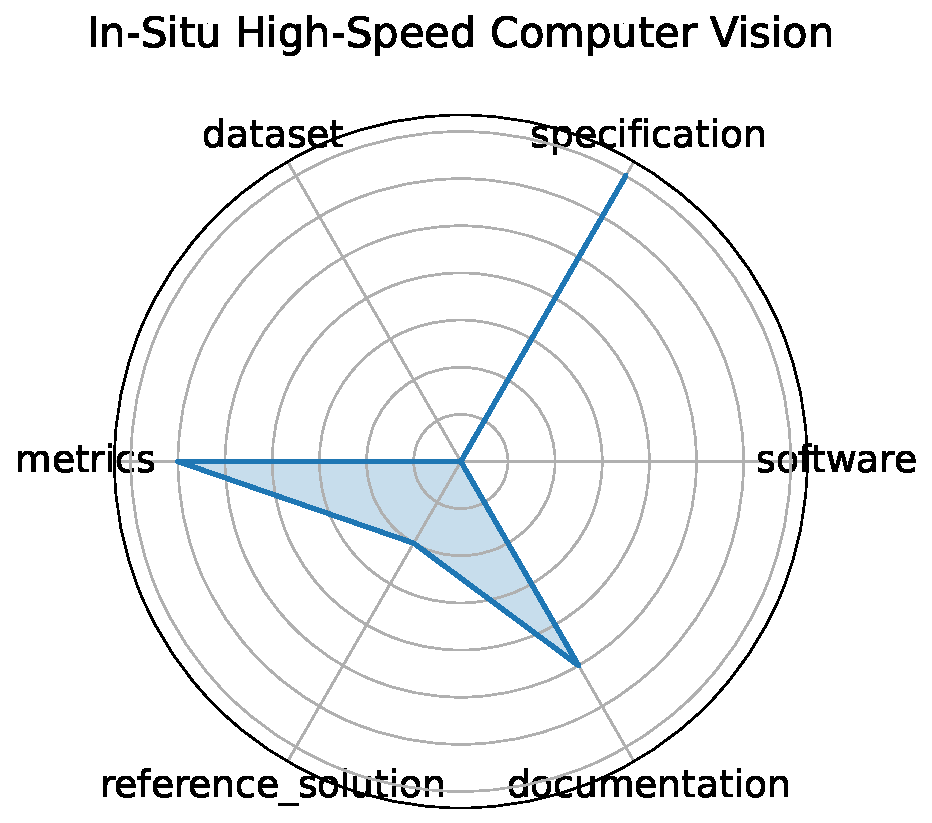
\includegraphics[width=0.2\textwidth]{in-situ_high-speed_computer_vision_radar.pdf}
}}
\clearpage